\chapter{Explotación}
\label{chapter:prod}

En los anteriores capítulos hemos descrito el proceso completo que hemos realizado con los datos: Los hemos localizado, los hemos limpiado, hemos creado diferentes modelos de minería de datos y hemos repetido estos pasos de manera iterativa. En este capítulo comentaremos el camino seguido para llevar los modelos construidos a un entorno productivo real.

Este paso que relata el viaje ``del laboratorio a la fábrica'', nos permitirá  cumplir el segundo objetivo planteado en la sección \ref{section:intro:objetivos} del documento: \textbf{extraer esta temática para nuevas llamadas en tiempo real}. Además como veremos en la sección \ref{section:prod:req} será necesaria para cumplir con otros requisitos propios de un sistema productivo.

\begin{figure}[!ht]
	\centering
	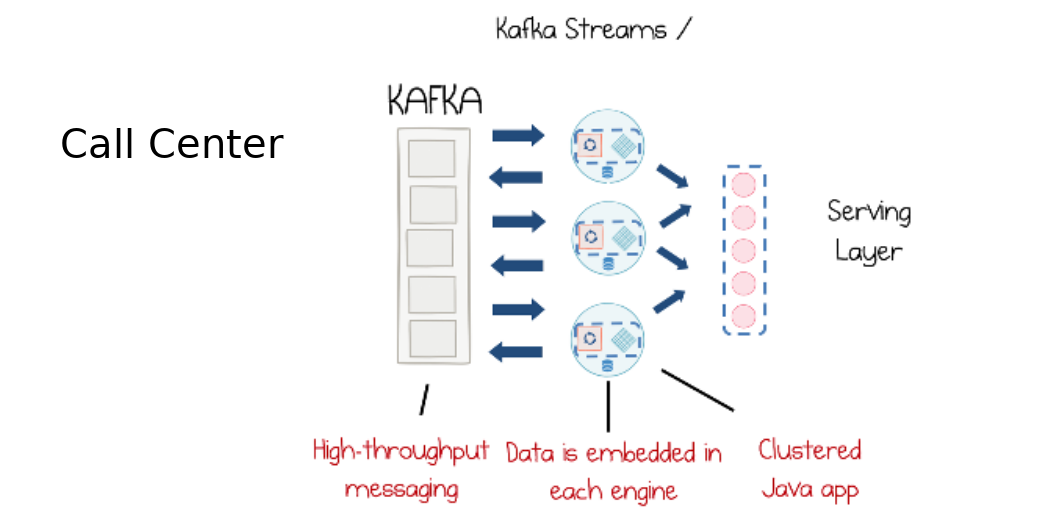
\includegraphics[width=1\textwidth]{images/exp/serving}
	\caption{Capa de \textit{streaming}}
	\label{fig:streamlayer}
\end{figure}


En la figura \ref{fig:streamlayer} podemos ver un \textit{zoom} de la capa de servicio de nuestra arquitectura que describiremos a lo largo del capítulo. 



\section{Requisitos del sistema productivo}
\label{section:prod:req}

En esta primera sección, antes de empezar con la definición de la capa de \textit{streaming}, vamos a recapitular los requisitos que deberá cumplir el sistema encargado de clasificar las llamadas recibidas del \textit{call center} en tiempo real. 

\begin{itemize}
	\item \textbf{Tiempo real}: El sistema debe ser capaz de clasificar las llamadas en tiempo real con una latencia máxima del orden de segundos. 
	\item \textbf{Escalabilidad}: El sistema debe poder escalar horizontalmente de modo que pueda responder en un futuro a un número de llamadas mayor. 
	\item \textbf{Alta disponibilidad}: El sistema debe estar siempre disponible sin que exista en el mismo un punto único de fallo (SPOF , \textit{Single Point Of Failure}).
	\item \textbf{Integración y despliegue continuos}: La integración y el despliegue del sistema deben ser continuos. Esto significa que una vez subido el código a un gestor de versiones deben poder realizarse de manera automática las pruebas necesarias, la compilación y el despliegue del sistema.
	
\end{itemize}

A lo largo del capítulo veremos como la aplicación cumple con los tres primeros puntos: tiempo real, escalabilidad y alta disponibilidad. El cuarto punto referente a la integración y el despliegue continuo se tratará de manera individual en el capítulo \ref{chapter:mant}.

\section{Arquitectura del sistema}


Al abordar la construcción del sistema hemos decidido usar una \textbf{arquitectura de microservicios}, cada uno de los cuales ejecute una parte del proceso. A la hora de diseñar estos microservicios hemos tenido en cuenta que cada uno ejecute una unidad de \textit{software} que tenga sentido por si misma y que pueda ser actualizada, sustituida o utilizada por terceros de una forma independiente. 

Una idea fundamental que subyace detrás de toda arquitectura de microservicios, es que cada microservicio desempeñe su tarea lo más aisladamente del resto y su comunicación con otros microservicios se realice usando protocolos simples y agnósticos a cualquier tecnología, usualmente el protocolo HTTP mediante API REST. 

Sin embargo el uso del protocolo HTTP tiene una serie de implicaciones que pueden no ser muy ventajosas para un sistema que requiere un procesamiento en tiempo real y que busca la simplicidad, como son la sincronía y y el acoplamiento con otros microservicios. La sincronía nos lleva a tener que ``preguntar'' constantemente a un microservicio sobre la existencia de nuevos datos, lo que, desde el punto de vista del rendimiento, implica que el \textit{thread} encargado del procesamiento deba esperar la respuesta HTTP antes de seguir con el procesamiento (esta perdida de rendimiento variará en función del tiempo de procesamiento necesario del microservicio llamado y de la latencia de la red).  Por otro lado, una arquitectura en la que los microservicios se comuniquen mediante REST implica un mínimo de acoplamiento, debido a que los microservicios deben conocer la existencia unos de otros, traduciéndose en una mayor complejidad a la hora de la orquestación de los mismos. 


Es por ello que una solución más optima para nuestro sistema consiste en combinar los beneficios de las arquitecturas \textit{event-driven} con los beneficios de los microservicios utilizando una \textbf{arquitectura de microservicios  \textit{event-driven} (EDM)}. Para desarrollar la arquitectura propuesta, necesitaremos un sistema de mensajería o \textit{streaming} por el que ``viajen'' los eventos y gracias al cual los microservicios puedan comunicarse entre sí. En nuestro caso hemos optado por utilizar \textbf{Apache Kafka como bus central de eventos}. 

El uso de Apache Kafka solventa los inconvenientes planteados por la arquitectura \textit{REST} eliminando la sincronía y el acoplamiento. Por un lado, los microservicios que tienen como origen un bus de mensajería son por naturaleza asíncronos, lo que implica que realizarán el procesamiento de los eventos en el momento que estos sean publicados en el bus; eliminando la necesidad de tener que ``preguntar'' por nuevos eventos y aumentando el rendimiento. Por otro lado, el uso de Apache Kafka hace que los microservicios estén totalmente desacoplados entre sí, eliminando la necesidad de que un microservicio conozca siquiera la existencia del resto. 

Además la arquitectura propuesta nos aporta otras características ventajosas para nuestro proyecto:

\begin{itemize}
	\item \textbf{Reprocesamiento}: Gracias a la capacidad de retención del bus, tenemos la posibilidad de reprocesar los mensajes pasados de ser necesario (p.e. para solventar errores de código).  
	\item \textbf{Alta disponibilidad}. El sistema es tolerante a fallos. Los datos se encuentran en el bus con un número de réplicas que evita la pérdida de los mismos ante caídas de nodos.
	\item \textbf{Escalabilidad}: Apache Kafka nos da la posibilidad de dividir nuestros \textit{topics} en particiones que pueden ubicarse en diferentes nodos. Esto nos proporciona escalabilidad horizontal tanto desde el punto de vista del almacenamiento como del cómputo.
	\item\textbf{ Soportar picos de carga}: Al existir una retención en el bus, en el caso de que ocurriese un pico en el número de eventos recibido que no puedan ser abordados por los procesadores, estos podrán ir procesando la información según su capacidad.
	\item \textbf{Evento en el centro}: Este tipo de arquitectura hace que diseñemos nuestras aplicaciones situando al evento, al dato, en el centro de nuestro sistema.
\end{itemize}


Sin embargo, aunque el uso de este tipo de microservicios  \textit{event-driven} (EDM) posea todas estas ventajas, es cierto que también hay que asumir que el uso de REST está muy implementado actualmente y muchas aplicaciones poseen un API REST \textit{out-of-the-box}. Esto nos llevará como veremos en el siguiente apartado a incorporar microservicios REST en nuestro modelo \textit{event driven}, creando en cierto modo una arquitectura híbrida.





\section{Microservicios}
En la sección anterior decidimos el modelo de arquitectura que vamos a utilizar para construir nuestro sistema, en esta sección nos centraremos en los microservicios que compondrán esa arquitectura.  

\subsection{Tecnología}
En el apartado \ref{section:arqu:tecn} hicimos un repaso por las tecnologías usadas en el proyecto, en este punto queremos tratar de profundizar con un poco más de detalle en las tecnologías que nos permitirán desarrollar y desplegar nuestros microservicios. Estas tecnologías son Kafka Streams y Tensorflow Serving.

\subsubsection{\textit{Kafka Streams}}

El núcleo de nuestra capa de \textit{Streaming} estará compuesto por microservicios desarrollados mediante 
 Kafka Streams. Kafka Streams \cite{kstreams} es una librería cliente que nos permite desarrollar aplicaciones y microservicios  cuya entrada y salida sea un bus Kafka. 
 
 Kafka Streams nos permite desarrollar aplicaciones en \textit{Java} (el lenguaje que usaremos) o Scala de una manera sencilla e intuitiva, además, a diferencia de otros \textit{frameworks} de procesamiento en tiempo real, como puede ser Spark Streaming, no tiene necesidad de disponer de un clúster aparte (usa el mismo bus Apache Kafka) lo que simplifica bastante nuestra arquitectura. Además Kafka Streams nos permitirá \textbf{garantizar la escalabilidad y la tolerancia a fallos} de nuestros despliegues. 
 
 Kafka Streams posee dos APIs diferentes: Processor API y  Streams DSL.  Processor API nos proporciona una capacidad a muy bajo nivel para definir la lógica de nuestro proceso \textit{streaming}; en cambio \textit{DSL}, que esta construido sobre  Processor API, nos permite de una manera sencilla, con un lenguaje declarativo, realizar la mayoría de operaciones posibles en un proceso de \textit{streaming}. Es por ello que en nuestros servicios utilizaremos principalmente \textbf{Streams DSL}, aunque en algún momento tengamos que recurrir a la Processor API para realizar tareas más avanzadas.
 
Una característica interesante de Streams DSL es la existencia de las denominadas KTables que nos permiten usar el Bus como si de una BBDD NoSQL Clave-Valor se tratara. Las Ktables utilizan un \textit{topic} de Apache Kafka, pero al acceder a ellas solo accedemos al último registro disponible para cada clave. Esta característica suele usarse sobre \textit{topics} compactos sin límite de retención, que son aquellos que periódicamente  borran las versiones antiguas de cada clave y retienen, de forma ilimitada, las versiones más recientes. Esta posibilidad nos permitirá cargar en el bus las tablas de \textit{lookup} necesarias para enriquecer registros en nuestro procesamiento y eliminará las dependencias de nuestro flujo con BBDD externas. 


 
 
\subsubsection{\textit{Tensorflow Serving}}

\textit{Tensorflow Serving} \cite{tfserving} está pensado para llevar a producción los modelos que hemos creado con \textit{Tensor Flow}, pudiéndose adaptar también para otros modelos. Tensorflow Serving nos permite desplegar nuestros modelos y algoritmos manteniendo intacta la API de consulta, esto lo hace ideal para entornos en los que queremos ir actualizando las versiones de nuestros modelos sin modificar el resto del sistema.

Los modelos desplegados con Tensorflow Serving pueden consultarse a través de un \textit{API} en C++ o mediante un \textbf{API REST} que es la opción escogida por nosotros debido a que, por la simplicidad del protocolo, es la que más encaja con nuestra arquitectura de microservicios. 

Una característica interesante de \textit{Tensorflow Serving}  es el \textbf{versionado}, ya que nos permite servir en paralelo varias versiones de un modelo, algo que puede ser muy interesante para, por ejemplo, realizar un test A/B.





\subsection{Microservicios}

Una vez determinada la arquitectura del sistema y las tecnologías escogidas para su implementación es el momento de diseñar los microservicios necesarios para nuestro caso de uso.

El primer paso es localizar las funciones básicas que queremos que realice nuestro sistema agrupadas en dos grandes etapas: preprocesamiento y predicción. La etapa de preprocesamiento será la encargada de preparar las llamadas para que puedan convertirse en la entrada de nuestro modelo, mientras que la etapa de predicción será la encargada de aplicar el modelo. 

Dentro de la etapa de preprocesamiento es necesario, en un primer lugar, la extracción de los \textit{tokens} de la transcripción de llamada, de esto se encargará un microservicio que hemos denominado \textit{\textbf{Tokenizer}}. Una vez obtenidos los \textit{Tokens} también será necesario, para que puedan convertirse en entrada del modelo, transformarlos en una secuencia numérica; esto será realizado por otro microservicio denominado \textit{\textbf{Sequencer}}.

Por último en la capa de predicción son necesarios otros dos pasos: por un lado aplicar el modelo  obteniendo una probabilidad de pertenencia a cada clase, de esto se encargará un microservicio denominado \textbf{\textit{tf-BajaFactura}} y, por otro lado, enriquecer estas predicciones con las etiquetas necesarias y enriquecer la salida del microservicio anterior; esto será responsabilidad de un microservicio denominado \textbf{\textit{Predicter}}. Como podemos imaginar por la definición, existirá un ligero acoplamiento entre estos dos microservicios, que comentaremos a lo largo de esta sección.
\vspace{0.2cm}

\begin{figure}[!ht]
	\centering
	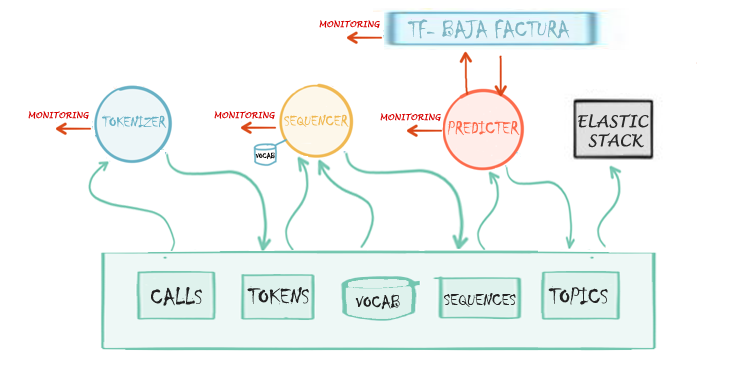
\includegraphics[width=1\textwidth]{images/exp/micro-arch-v3}
	\caption{Arquitectura microservicios}
	\label{fig:micro-arch}
\end{figure}


En la figura \ref{fig:micro-arch} podemos ver como los microservicios propuestos interactúan entre sí a través del bus, con excepción del microservicio  \textbf{\textit{tf-BajaFactura}}. Estos microservicios conforman la parte capa de \textit{streaming} de nuestro sistema. En el capítulo siguiente veremos como la salida de esta capa de \textit{streaming} alimentará la capa de servicio.


A continuación, en los siguientes subapartados describiremos uno a uno los diferentes microservicios. 


\subsection{\textit{Tokenizer}}

Este microservicio tiene como entrada las llamadas transcritas que llegan al bus en tiempo real. A partir del texto de las mismas el sistema inicia un proceso de \textit{tokenizacion} eliminando \textit{stopwords}, carácteres especiales (signos de puntuación, 'ñ's, acentos...), palabras comunes, números, nombres propios y pasando a minúscula cada uno de los tokens.  El proceso de \textit{tokenización} pretende ser lo más fiel posible al proceso realizado en \textit{Python} durante la etapa de entrenamiento del modelo.

Una vez obtenida la lista de \textit{tokens} esta se vuelve a disponibilizar en el bus en un nuevo \textit{topic}. Este nuevo \textit{topic} con las llamadas \textit{tokenizadas} puede ser de utilidad no solo para nuestro sistema, si no también para cualquier otro sistema de análisis de texto que necesite partir de los datos \textit{tokenizados}.

El \textit{topic} de entrada del microservicio  \textit{Tokenizer}, llamado \textit{CALLS}, tendrá como clave el código de la llamada y como cuerpo un objeto \textit{json} con los siguientes campos:

\begin{itemize}
		\item \textbf{\textit{co\_verint}} : Código de la llamada. 
		\item  \textbf{\textit{call\_text}} : Texto de la llamada. 
		\item  \textbf{\textit{call\_timestamp}}: Hora de la llamada.
        \item \textbf{\textit{province}}: Provincia desde la que se ha realizado la llamada. 
        \item \textbf{\textit{co\_province}}: Código de provincia desde la que se ha realizado la llamada. 
        \item \textbf{\textit{duration}}: Duración en segundos de la llamada. 
        \item \textbf{\textit{control\_type}}: De existir, tipo de llamada (usado para el proceso de verificación). 
\end{itemize} 

Como salida escribirá en un \textit{topic}  llamado \textit{TOKENS.CALLS} un evento cuya clave será el código de la llamada y cuyo cuerpo un objeto \textit{json} con los siguientes campos:

\begin{itemize}
		\item \textbf{\textit{co\_verint}} : Código de la llamada. 
		\item  \textbf{\textit{call\_text}} : Texto de la llamada. 
		\item  \textbf{\textit{call\_timestamp}}: Hora de la llamada.
        \item \textbf{\textit{province}}: Provincia desde la que se ha realizado la llamada. 
        \item \textbf{\textit{co\_province}}: Código de provincia desde la que se ha realizado la llamada. 
        \item \textbf{\textit{duration}}: Duración en segundos de la llamada. 
        \item \textbf{\textit{control\_type}}: De existir, tipo de llamada (usado para el proceso de verificación).  
        \item \textbf{\textit{tokens}}: Lista de tokens extraída de \textit{call\_text}. 
\end{itemize} 



\subsection{\textit{Sequencer}}
Este microservicio toma como entrada la salida del microservicio anterior y a partir de la lista de \textit{tokens} devuelve una secuencia de tamaño fijo determinado $T$. Para ello, utiliza un diccionario en el que cada \textit{token} se corresponde con un número, utilizando el $0$ para \textit{tokens} que no existan en este diccionario. Esta secuencia esta limitada a un tamaño determinado $T$, por lo que llamadas con un número mayor de $tokens$ son recortadas y se utiliza \textit{padding} por la izquierda para completar la secuencia de llamadas con un tamaño menor a $T$.

El diccionario ha sido calculado sobre el conjunto de datos de  entrenamiento y contiene el vocabulario del modelo. Este diccionario contiene como clave todos los \textit{tokens} posibles y como valores el identificador usado para cada \textit{token}. La lectura del mismo se realiza desde el mismo bus, utilizando la funcionalidad \textit{KTable} de \textit{Kafka Streams}.


Una vez obtenida la secuencia de caracteres, esta se disponibiliza en un nuevo \textit{topic} del bus. Además de por nuestro sistema, este valor puede ser consumido por otros microservicios o sistemas que tengan como objetivo aplicar diferentes modelos a las secuencias obtenidas.

El \textit{topic} de entrada del microservicio \textit{Sequencer} será el topic  \textit{TOKENS.CALLS} descrito en el apartado anterior. 

Como salida escribirá en un \textit{topic}  llamado \textit{SEQUENCES.CALLS} un evento cuya clave será el código de la llamada y cuyo cuerpo un objeto \textit{json} con los siguientes campos:

\begin{itemize}
		\item \textbf{\textit{co\_verint}} : Código de la llamada. 
		\item  \textbf{\textit{call\_text}} : Texto de la llamada. 
		\item  \textbf{\textit{call\_timestamp}}: Hora de la llamada.
        \item \textbf{\textit{province}}: Provincia desde la que se ha realizado la llamada. 
        \item \textbf{\textit{co\_province}}: Código de provincia desde la que se ha realizado la llamada. 
        \item \textbf{\textit{duration}}: Duración en segundos de la llamada. 
        \item \textbf{\textit{control\_type}}: De existir, tipo de llamada (usado para el proceso de verificación).  
        \item \textbf{\textit{sequence}}: Lista de 866 enteros en el que cada uno representa el identificador de un \textit{token}. La secuencia se completa con ceros en caso de ser necesario.
\end{itemize} 


Además se apoyará en un topic compacto que no tendrá  límite de retención, denominado \newline \textit{TBL.VOCABULARY.CALLS}, cuya clave son los \textit{tokens} existentes en el vocabulario y,  cuyo  valor es un identificador para cada uno de ellos.

\subsection{\textit{tf-BajaFactura}}
\textit{\textbf{tf-BajaFactura}} quizás sea el microservicio más tradicional y discordante de los que vamos a utilizar en nuestro sistema debido a que este microservicio se encuentra totalmente desacoplado del bus y del resto de microservicios. Mediante un API REST aplica nuestro modelo de TensorFlow a una o varias secuencias de entradas y, para cada secuencia, devuelve la probabilidad de pertenencia a las clases: ``Baja'', ``Factura'' y ``Resto''.

El motivo principal para usar API REST en este microservicio se debe al uso de la tecnología  Tensorflow Serving comentada en el capítulo anterior y que nos permite con mucha facilidad desplegar nuevos modelos y algoritmos, manteniendo la misma estructura en el servidor y la misma API. Además su integración es automática con los modelos generados con TensorFlow (con o sin Keras). Esta decisión permite a los \textit{data-scientist} desplegar nuevas versiones de sus modelos, ya sea por degradación o por mejora, mientras el resto del flujo permanece inalterable. 

La entrada del modelo \textit{tf-BajaFactura} será un documento \textit{json} que contenga el campo \textit{instances} compuesto por una lista de secuencias. En nuestro caso una sola secuencia, ya que el modelo será llamado con cada evento recibido. La salida será también en \textit{json} y contendrá una lista de predicciones, en cada predicción tendremos la probabilidad de pertenencia a cada clase.




\subsection{Predicter}
Este último microservicio tiene como entrada el \textit{topic} generado por \textit{\textbf{Sequencer}} y a partir del mismo realiza una llamada a \textit{\textbf{tf-BajaFactura}}. Una vez obtenidas las predicciones, las enriquece con las etiquetas necesarias. Además en el caso de existir un atributo de control comprueba si la predicción ha sido correcta, esto nos servirá para validar la eficiencia del modelo a lo largo del tiempo. 

Como podemos observar, es el único microservicio que tiene una dependencia con otro (\textit{tf-BajaFactura}), sin embargo la API de un modelo implementado con Tensorflow Serving \cite{tfserving} es siempre idéntica. Esto provoca que la llamada no varíe aunque cambie el modelo. Además, en el servicio \textit{\textbf{Predicter}}, el número de clases y las etiquetas de las mismas son configurables , pudiendo  reutilizarse este microservicio para cualquier servicio predictivo desplegado mediante  Tensorflow Serving.

La salida de este microservicio es publicada en un nuevo \textit{topic} en el bus, esta información puede ser de utilidad para diversos sistemas que quieran realizar analítica en función de la temática de las llamadas o que quieran visualizarla. Nosotros la usaremos en nuestra capa de servicio que describiremos en el siguiente capítulo.

El \textit{topic} de entrada del microservicio \textit{Predicter} será el topic  \textit{SEQUENCES.CALLS} descrito en el servicio \textit{Sequencer}. 


Como salida escribirá en un \textit{topic}  llamado \textit{TOPICS.CALLS} un evento cuya clave será el código de la llamada y cuyo cuerpo un objeto \textit{json} con los siguientes campos:

\begin{itemize}
		\item \textbf{\textit{co\_verint}} : Código de la llamada. 
		\item  \textbf{\textit{call\_text}} : Texto de la llamada. 
		\item  \textbf{\textit{call\_timestamp}}: Hora de la llamada.
        \item \textbf{\textit{province}}: Provincia desde la que se ha realizado la llamada. 
        \item \textbf{\textit{co\_province}}: Código de provincia desde la que se ha realizado la llamada. 
        \item \textbf{\textit{duration}}: Duración en segundos de la llamada. 
        \item \textbf{\textit{control\_type}}: De existir, tipo de llamada (usado para el proceso de verificación).  
        \item  \textbf{\textit{predictions}}: Lista con las predicciones devueltas por el servicio  \textit{tf-BajaFactura}. 
        \item  \textbf{\textit{error}}: De producirse, contendrá el error devuelto por el  servicio  \textit{tf-BajaFactura} o el error de conexión con el mismo.      
         \item  \textbf{\textit{model}}: ID del modelo aplicado, en nuestro caso siembre será BajaFactura.
         \item  \textbf{\textit{pred\_type}}: Etiqueta de la clase más probable según la predicción.
         \item  \textbf{\textit{control\_success}}: En el caso de existir el campo \textit{control\_type}, \textit{Booleano} que nos indica si la predicción ha sido correcta.
\end{itemize} 


\section{Monitorización de Microservicios}

Si bien es cierto que el hecho de utilizar una arquitectura orientada a eventos, aparte de la sencillez intrínseca de nuestro sistema, nos simplifica en cierto modo la orquestación de nuestro servicios y nos permite prescindir de herramientas de APM (\textit{Application Performance Monitoring}); una monitorización del desempeño de nuestros microservicios es siempre necesaria, tanto para garantizar el correcto funcionamiento de los mismos y poder detectar posibles puntos de fallo, como para detectar pérdidas de rendimiento en cualquier punto del sistema. 

En esta sección veremos los métodos utilizados para monitorizar los microservicios dependiendo de su tecnología. 


\subsection{Servicios \textit{Kafka Streams}}

Los servicios de Kafka Streams corren sobre la máquina virtual de Java lo que nos permite tener acceso a sus métricas por medio de la JMX(\textit{Java Management Console}). Ademas Confluent posee una documentación de los MBeans y de las métricas que contienen en su documentación oficial \cite{monitoringstreams}. 


El inconveniente de estas métricas es que tienen que extraerse por medio de protocolos RMI (\textit{Java Remote Method Invocation}) lo que complica su explotación, sin embargo a partir de la versión 6 del JDK (\textit{Java Development Kit}) tenemos la posibilidad de exportar estas métricas de JMX directamente mediante API REST. Esto nos da la posibilidad de poder recolectar las métricas directamente mediante una llamada HTTP.

Para recolectar estás métricas utilizaremos los Beats de  Elastic, concretamente Metricbeat. Este será el encargado de recolectar las métricas necesarias y enviarlas a Logstash para su posterior almacenamiento en Elasticsearch. El flujo de Logstash a Elasticsearch lo trataremos con más detalle en el próximo capítulo en el que veremos la capa de servicio, ya que las métricas de monitorización seguirán el mismo recorrido que los datos de clasificación. 


De todas las métricas disponibles de Confluent, nosotros extraeremos con una frecuencia de un minuto las siguientes métricas:

\begin{itemize}
	\item \textit{mbean 'java.lang:type=Runtime'} : Métrica \textit{Uptime}.
	
	\item \textit{mbean 'kafka.streams:type=stream-metrics'}: Métricas \textit{process-latency-avg}, \textit{process-latency-max} y \textit{process-rate}.
\end{itemize}



Esto nos permitirá para cada microservicio tener información del tiempo de servicio del mismo, de la latencia máxima y media de procesamiento de los eventos y de la tasa de procesamiento. 





\subsection{Servicios \textit{Tensorflow Serving}}

En el caso de la monitorización del servicio \textit{tf-BajaFactura}, habilitaremos la monitorización de Prometheus de Tensorflow Serving para que las métricas sean accesibles mediante API REST, pero en lugar de utilizar Prometheus (para no incluir complejidad en nuestro sistema), usaremos directamente el \textit{Input} \textit{Http\_poller} de Logstash.

De todas las métricas disponibles en Tensorflow Serving nos quedaremos unicamente con: 

\begin{itemize}
\item \textbf{Estado}: Que nos dará información sobre si el modelo ha sido cargado con éxito y se encuentra operativo.  

\item \textbf{Total peticiones}: Total de peticiones resueltas por el modelo.

\item \textbf{Total nanosegundos del grafo}: El total de tiempo que el modelo ha dedicado en procesar todas las peticiones. Utilizaremos el total de peticiones para extraer la latencia media y lo expresaremos en milisegundos. 

\end{itemize}




Una vez recolectadas las métricas y enviadas a Logstash, seguirán el mismo flujo descrito en el apartado anterior hacia la capa de servicio, este flujo será tratado en más detalle en el capítulo siguiente. 

Además de las métricas recolectadas, la monitorización del microservicio \textit{\textbf{predicter}} nos dará información combinada de ambos ya que internamente realiza una llamada a \textit{tf-BajaFactura}.



\section{Inyector: simulador de tiempo real}
Como ya hemos comentado en anteriores capítulos actualmente las transcripciones de las llamadas no se encuentran disponibles en tiempo real, es por ello que se ha diseñado un inyector de llamadas.

Este inyector, realizado en Python utiliza como fuente la transcripción de las llamadas realizadas en batch. Y a partir de la misma cumplirá los siguientes objetivos: 

\begin{itemize}
	\item \textbf{ Extraer la frecuencia de llamadas por hora}. De este modo simularemos el comportamiento real de un \textit{call-center} inyectando más llamadas a las horas del día con mayor actividad.
	\item \textbf{Multiplicar el número de llamadas}. Teniendo en cuenta que actualmente solo se transcriben un 4\% del total de las llamadas, el inyector multiplicará por 25 el número de llamadas recibidas en un día para simular el comportamiento real de un sistema que ingeste el 100\% de las llamadas.
	\item \textbf{Introducir datos de control}: El inyector insertará en un porcentaje de llamadas los datos reales de clasificación con el fin de poder verificar el comportamiento del modelo. En un entorno real se podrían insertar periódicamente un número de llamadas de control que nos permitan este objetivo.
	
\end{itemize}

Una vez realizadas estas tareas, el inyector publicará todas las llamadas al bus, simulando un comportamiento real. De este modo las llamadas estarán disponibles en tiempo real para cualquier consumidor que las necesite.

Aunque el inyector podría verse como un microservicio más, hemos preferido dejarlo fuera del sistema a lo largo de todo el apartado, debido a que lo consideramos una pieza auxiliar que nos permite simular el comportamiento real del sistema sin disponer de los datos en este momento.

